\documentclass[12pt,a4paper]{article}
\usepackage[utf8]{inputenc}
\usepackage{amsmath,enumitem,amsfonts,amssymb,graphicx}
\usepackage{multicol}
\usepackage{sectsty}
\graphicspath{ {./} }
\usepackage{scrextend}

\usepackage[%
    left=1.0in,%
    right=1.0in,%
    top=0.8in,%
    bottom=1.0in,%
]{geometry}%

\sectionfont
{\fontsize{14.4}{12}\selectfont}
\title{\textbf{Principles of AI Planning
		\\{\Large Exercise Sheet 5}}}
\date{29.11.2019}

\makeatletter
\renewcommand{\@maketitle}
{
	\newpage
	\null
	\vskip 2em%
	\begin{center}%
		{\LARGE \@title \\ \par}%
	\end{center}%
	\par
} \makeatother


\begin{document}
	\begin{flushleft}
		Authors:\\
		Erick Rosete Beas | er165@uni-freiburg.de\\
		Jessica Lizeth Borja Diaz | jb986@uni-freiburg.de\\
	\end{flushleft}
	{\let\newpage\relax\maketitle}
	\begin{center} 
		\large 29.11.2019 
	\end{center}

\hfill\break
\section*{Exercise 5.1: A* search}
	\textbf{a) Solve the puzzle with the A* algorithms}\\
	\begin{center}
		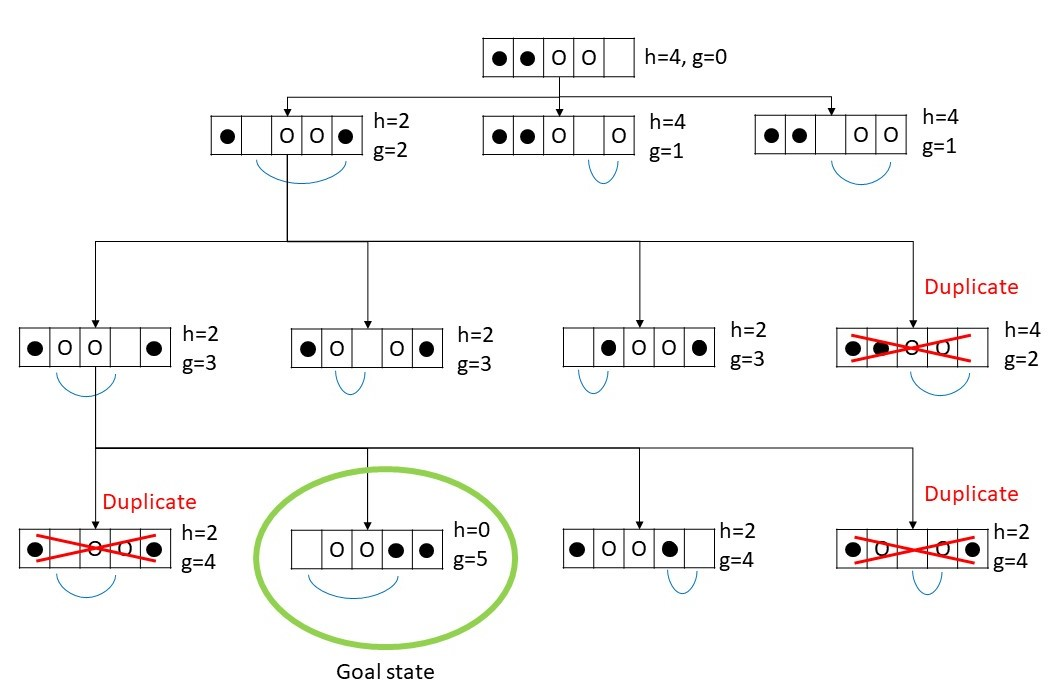
\includegraphics[scale=0.4]{A_star_0.jpg}\\
		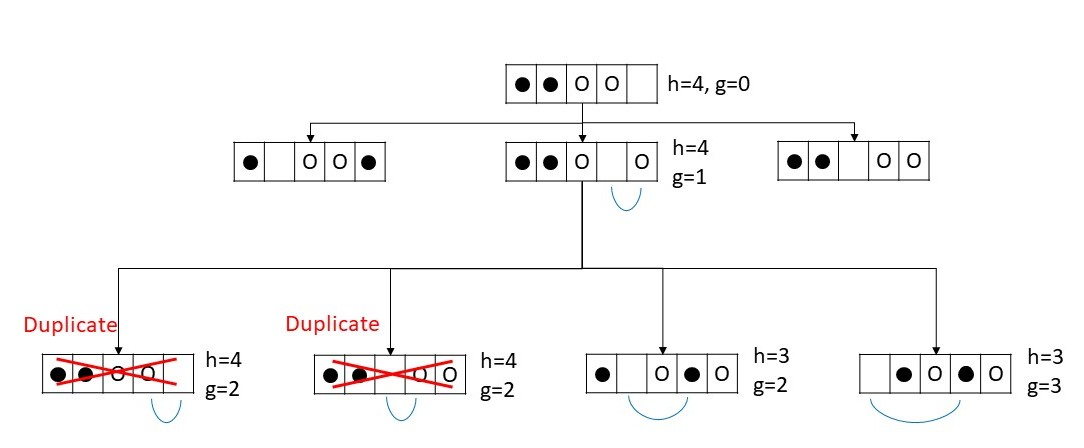
\includegraphics[scale=0.4]{A_star_1.jpg}\\
		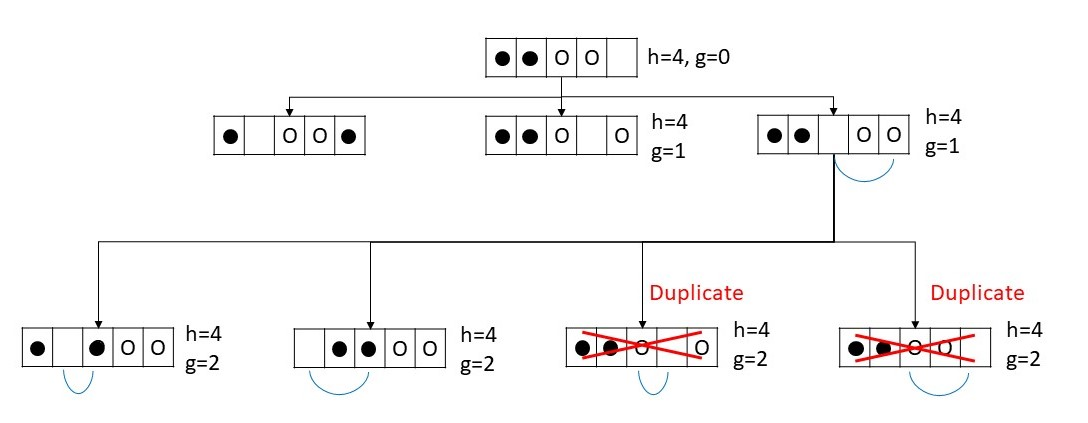
\includegraphics[scale=0.4]{A_star_2.jpg}\\
	\end{center}
	\textbf{b) show that h is admissible}
	\begin{addmargin}[1em]{1em}% 1em left, 2em right
		\quad Given an initial state with a black tile to the left of a white
		tile, the only way that a black tile can reach the goal state is if
		it jumps this white tile. The cost of jumping over one tile is 
		at least 1, and if it jumps over two tiles then the cost is 2. 
		This means that the cost of each black tile, to reach the right end,
		is at least the number of white tiles to the right, which is 
		precisely our heuristic. Therefore $h(s) \leq h^*(s) $
		then the heuristic is \emph{admissible}
	\end{addmargin}

%%%%%%%%%%%%%%%%%%%%%% Exercise 5.2 %%%%%%%%%%%%%%%%%%%%%%%%%%%%%
\section*{Exercise 5.2: Enforced hill-climbing}
\begin{enumerate}[label=\alph*)]
	\item \textbf{For each invocation of the 
			\texttt{improve} procedure, specify
			the state after improvement by giving the new coodinates}
	\item \textbf{Record the solution plan}
\end{enumerate}
\end{document}